\documentclass[20 pts]{article}
\usepackage{xeCJK}
\usepackage{amsfonts}
\usepackage{amssymb}
\usepackage{amsmath}
\usepackage{bm}
\setCJKmainfont{SimSun}
\title{Turbo Codes and Turbo Decoding}
\author{Kwame Ackah Bohulu}
\date{20-04-2017}
\begin{document}
\maketitle


\section{Introduction}
A typical Turbo encoder is formed fom two convolutional encoders, and an interleaver. The two convolutional encoders, also known as component encoders are connected in parallel via the interleaver. It was discovered by Claude Berrou and introduced to the scientific community in 1993[2]. In the usual case, two identical convolutional encoders are used. The order of the information sequence is rearranged via an interleaver before being fed into the second convolutional interleaver. The interleaver in the turbo encoder is used to reduce the number of low-weight codewords. The minimum achievable output rate of the interleaver is 1/3 but can be increased to 1/2 or 2/3 via puncturing. Turbo codes achieve excellent performance at low signal to noise ratios and have been used in many applications including mobile telephony standards. In this research paper, a brief introduction to turbo codes followed by the principle behind the construction of turbo codes are given in section 2 and 3 respectively. A detailed explanation of the  BCJR algorithm and its application in the iterative decoding is given in section 4. Finally in section 5, the system model used in the simulation of the turbo code is explained in detail.


\section{Convolution Codes}
Convolutional codes are foremed by feeding an information sequence into finite state shift registers[1]. In general, the shift register consists of $K$ stages each containing $k$ bits and $n$ linear algebraic function generators, where $K $is the constraint length of the shift register, $k $is the number of input bits fed into the shift register at a go,and $n$ is the number of bits present at the output of the shift register. The rate of the convolutional encoder is $\frac{k}{n}$. The linear algebraic function generator perform modulo 2 addition. The generator function of the convolutional encoder is made up of n vector each of size Kk. Various representations of genetator matrix are shown below.

\paragraph{}
K=3,k=1,n=3\newline
$g_1=[1 0 0], g_2=[1 0 1], g_3=[1 1 1]$\newline
octal form =(4, 5, 7)\newline
$c^{(1)}=u*g_1,c^{(2)}=u*g_2,c^{(3)}=u*g_3$\newline
Output code sequence=$(c_1^{(1)},c_1^{(2)},c_1^{(3)},c_2^{(1)},c_2^{(2)},c_2^{(3)},...)$
\paragraph{}
D domain\newline
$U(D)=\sum_{i=0}^{\infty} u_iD^i $\newline
$g_1(D)=1,g_2(D)=1+D^2,g_3(D)=1+D+D^2$\newline
$C^{(1)}(D)=U(D)g_1(D),C^{(2)}(D)=U(D)g_2(D),C^{(3)}(D)=U(D)g_3(D)$\newline
$C(D)=C^{(1)}(D^3)+DC^{(2)}(D^3)+D^2C^{(3)}(D^3)$
\paragraph{}
Convolutional codes are best described using a trellis graph. The number of nodes contained in the trellis is eqivalent to the number of possible states of the shift register. for a general rate$\frac{k}{n}$ code with constraint length $K$ , the trellis has $2^{k(K-1)}$ossible nodes with $2^k$ branches entering and leaving each node. 
\subsubsection{Recursive Systematic and Nonrecursive Systematic Convolutional Codes}
Convolutional codes which have the information sequence as part of the code are known as systematic convolutional codes. Futhermore, a convolutional code constructed by the use of a feedback shift register is known as a recursive convolutional code. It should be noted that recursive convolutional code are always sytematic whiles nonrecursive convolutional codes are often non-systematic. Also, the generator matrix for systematic convolutional codes contain a polynomial matrix.
\paragraph{}
rate=1/2, K=3, $g_1=[1 1 1]$, $g_2=[1 0 1]$\newline
G=[1 $g_2$/$g_1$]\paragraph{}
The ''1'' in the generator matrix signifies the systematic portion of the code whiles denominator and numerator signifies the feedback input and the output respectively. Recursive systematic encoders are used as component codes in most Turbo code applications.
\section{Turbo Encoder}
As was mentioned earlier, a turbo encoder is made up of two recursive systematic convolutional(RSC) encoders connected in parallel by an interleaver[4]. The choice of interleaver is very important, as it caused a reduction in the  number of low-weight codewords(called the multiplicity)[3],[5]. Due to the huge number of states that exist in the turbo encoder, maximum likelihood decoding is impossible. Instead, the turbo decoding algorithm, which is based on the BCJR algorithm is used.
\section{BCJR Algorithm}
The BCJR algorithm was invented by Bahl, Cocke,Jelinek and Raviv in 1974. Rather than searching for the most likely input sequence, this algorithm uses the MAP algorithm to decode each input sequence. in order to explain the BCJR algorithm, the following assumptions are made\newline
1. The information sequence length, \textbf{u}is $N$,\textbf{u}=$\{u_1,u_2,....,u_N\}$\\
In the case where ,$k=1$, $u_i\in \{0,1\}$\newline
2. The encoded sequence length \textbf{c}is $N$,\textbf{c}=$\{c_1,c_2,....,c_N\}$\\
and the length of$c_i$ is $n$.\newline
3.The encoded sequence is transmitted through an AWGN channel and the received sequence \textbf{y}is real and has length $n$.\textbf{y}=$\{y_1,y_2,....,y_N\}$\paragraph{}
The BCJR algorithm calculates the a posteriori LLR,$L(u_i|y)$ and returns an estimate of the original information sequence using the equation below.\begin{equation}L(u_i|y)=\ln\frac{P(u_i=1|\boldsymbol{y})}{P(u_i=0|\boldsymbol{y})}\end{equation}
The calculation of the BCJR algorithm is made easier by the use of a trellis graph。At time $i$, the current state is given as $\sigma_i=s$ and the previous state is given by $\sigma_{i-1}=s'$. The received symbol at the decoder at time $i$, is given by $y_i$. Before time $i$,$i-1$ symbols would have been received and after time $I$ $N-i$ symbols will be received. From the above intuition, the total received sequence \textbf{y} at time $i$ can be divided in past present and future subsequences、$$\boldsymbol{y}=\boldsymbol{y}_{<i} \boldsymbol{y}_{i} \boldsymbol{y}_{>i}$$
From the trellis graph, we note that the transition from $\sigma_{i-1}=s'$ to $\sigma_i=s$ is determined by the value of $u_i$ .Since state transitions are mutually exclusive, the probability that a transition will occur is the sum of the respective probabilities.
$$\therefore P(u_i=1|\boldsymbol{y})=\sum_{R_1}^{}P(s',s|\boldsymbol{y})$$
$$P(u_i=0|\boldsymbol{y})=\sum_{R_0}^{}P(s',s|\boldsymbol{y})$$
where\\ $R_0$ is the set  transition from $\sigma_{i-1}=s'$ to $\sigma_i$=s as a result of $u_i=0$\\
$R_1$ is the set  transition from $\sigma_{i-1}=s'$ to $\sigma_i$=s as a result of $u_i=1$\\
\paragraph{}
substituting \textbf{y},$P(u_i=1|\boldsymbol{y})$ and $P(u_i=0|\boldsymbol{y})$ into equation 1、
\begin{equation}
\begin{split}
L(u_i|y)&=\ln\frac{\sum_{R_1}^{}P(s',s|\boldsymbol{y})}{\sum_{R_0}^{}P(s',s|\boldsymbol{y})}\\
&=\ln\frac{\sum_{R_1}^{}P(s',s,\boldsymbol{y})}{\sum_{R_0}^{}P(s',s,\boldsymbol{y})}\\
&=\ln\frac{\sum_{R_1}^{}P(s',s,\boldsymbol{y}_{<i} \boldsymbol{y}_i \boldsymbol{y}_{>i})}{\sum_{R_0}^{}P(s',s,\boldsymbol{y}_{<i} \boldsymbol{y}_i \boldsymbol{y}_{>i})}
\end{split}
\end{equation}
from Bayes equation
\begin{equation}
\begin{split}
P(s',s,\boldsymbol{y}_{<i} \boldsymbol{y}_i \boldsymbol{y}_{>i})&=P(\boldsymbol{y}_{>i}|s',s,\boldsymbol{y}_{<i}\boldsymbol{y}_{i})P(s',s,\boldsymbol{y}_{<i}\boldsymbol{y}_{i})\\
&=P(\boldsymbol{y}_{>i}|s)P(\boldsymbol{y}_{i},s|s',\boldsymbol{y}_{<i})P(s',\boldsymbol{y}_{<i})\\
&=P(\boldsymbol{y}_{>i}|s)P(\boldsymbol{y}_{i},s|s')P(s',\boldsymbol{y}_{<i})\\
&=\alpha_{i-1}(s')\gamma_i(s',s)\beta_i(s)
\end{split}
\end{equation}
$\alpha_{i-1}(s')=P(s',\boldsymbol{y}_{<i})$ represent the joint probability that at time $i-1$、the state $s'$ and the received sequence untill then is $\boldsymbol{y}_{<i}$.\\
$\gamma_i(s',s)=P(\boldsymbol{y}_{i},s|s')$ represents the probability that the next state is $s$ and the received symbol is $\boldsymbol{y}_{i}$ given that the previous state is $s$.\\
$\beta_i(s)=P(\boldsymbol{y}_{>i}|s)$ represents the conditional probability tha given the current state, $s$, the future sequence will be $\boldsymbol{y}_{>i}$
Substituting equation 3 into equation 1 yields the equation below.
\begin{equation}L(u_i|y)=\ln\frac{\sum_{R_1}^{}\alpha_{i-1}(s')\gamma_i(s',s)\beta_i(s)}{\sum_{R_0}^{}\alpha_{i-1}(s')\gamma_i(s',s)\beta_i(s)}\end{equation}
\subsection{Calculation of $\gamma_i(s',s)$}
$\gamma_i(s',s)$ is given by the equation below.
\begin{equation}
\begin{split}
\gamma_i(s',s)&=P(\boldsymbol{y}_{i},s|s')\\
&=P(\boldsymbol{y}_{i}|s',s)P(s|s')\\
&=P(\boldsymbol{y}_{i}|c_i)P(u_i)
\end{split}
\end{equation}
In the case of the AWGN channel、
\begin{equation}
\gamma_i(s',s)=\frac{P(u_i)}{(\pi N_o)^{n/2}}exp(-\frac{\|{y_i-c_i}\|^2}{N_o})
\end{equation}
\subsection{Calculation of $\alpha_{i-1}(s')$}
$\alpha_{i-1}(s')=P(s',\boldsymbol{y}_{<i})$. This equation can be re-written as、
\begin{equation}
\begin{split}
\alpha_{i}(s)&=P(s,\boldsymbol{y}_{<i+1})\\
&=P(s,\boldsymbol{y}_{<i},\boldsymbol{y}_{i})
\end{split}
\end{equation}

From probability theory,
\begin{equation}
P(A)=\sum_{B}^{}P(A,B)\\
\end{equation}

\begin{equation}
\begin{split}
\therefore \alpha_i(s)&=\sum_{s'}^{}P(s,\boldsymbol{y}_{i}|s',\boldsymbol{y}_{<i})P(s',\boldsymbol{y}_{<i})\\
&=\sum_{s'}^{}P(s,\boldsymbol{y}_{i}|s')P(s',\boldsymbol{y}_{<i})\\
&=\gamma_i(s',s)\alpha_{i-1}(s')
\end{split}
\end{equation}
	In the case of an all-zero terminated trellis、the initial conditions for $\alpha_i(s)$ are

\[
    \alpha_i(s)= 
\begin{cases}
   1,& s= 0\\        0,              &  s\neq 0
\end{cases}
\]

\subsection{Calculation of $\beta_i(s)$}
$\beta_i(s)=P(\boldsymbol{y}_{>i}|s)$
This can be re-written as
\begin{equation}
\begin{split}
\beta_{i-1}(s')&=P(\boldsymbol{y}_{>i-1}|s')\\
&=\sum_{s}^{}P(\boldsymbol{y}_{>i}|s',s,\boldsymbol{y}_{i})P(s,\boldsymbol{y}_{i}|s')\\
&=\sum_{s}^{}P(\boldsymbol{y}_{>i}|s)P(s,\boldsymbol{y}_{i}|s')\\
&=\beta_i(s)\gamma_i(s',s)
\end{split}
\end{equation}

In the case of an all-zero terminated trellis、the initial conditions for $\beta_i(s)$ are

\[
    \beta_N(s)= 
\begin{cases}
   1,& s= 0\\        0,              &  s\neq 0
\end{cases}
\]
\subsection{Log-MAP and Max-Log-MAP}
For the BCJR Algorithm、when the trellis length is very long、it becomes numerically unstable. In such cases, the log domain versions of the BCJR algorithm、Log-MAP andMax-Log-MAPAlgorithm are used instea. In the case of Log-MAP the following definitions are used.

\begin{equation}
\begin{split}
&\widetilde{\alpha}_i(s)=\ln(\alpha(s))\\
&\widetilde{\beta}_i(s)=\ln(\beta(s))\\
&\widetilde{\gamma}_i(s',s)=\ln(\gamma(s',s))
\end{split}
\end{equation}
The forward($\widetilde{\alpha}_i(s)$) and backward($\widetilde{\beta}_{i-1}(s)$) recursions as well as the LLR are calculated using the equations below.
\begin{equation}
\begin{split}
&\widetilde{\alpha}_i(s)=\ln\sum_{s'}^{}\exp(\widetilde{\alpha}_{i-1}(s')+\widetilde{\gamma}(s',s))\\
&\widetilde{\beta}_{i-1}(s)=\ln\sum_{s}^{}\exp(\widetilde{\beta}_{i}(s')+\widetilde{\gamma}(s',s))\\
&L(u_i)=\ln\Big[\sum_{R_1}^{}\exp(\widetilde{\alpha}_{i-1}(s')+\widetilde{\gamma}(s',s)+(\widetilde{\beta}_{i}(s'))\Big]-\ln\Big[\sum_{R_0}^{}\exp(\widetilde{\alpha}_{i-1}(s')+\widetilde{\gamma}(s',s)+(\widetilde{\beta}_{i}(s'))\Big]
\end{split}
\end{equation}
In order to increase calculation efficiency、Max-Log-MAP algorithm is used. The following definitions are used.
\begin{equation}
\begin{split}
&\max{*}\{x,y\}\triangleq \ln(e^x+e^y)\\
&\max{*}\{x,y,z\}\triangleq \ln(e^x+e^y+e^z)
\end{split}
\end{equation}

With the above notations, The forward and backward recursions as well as the LLR are calculated using the equations below.

\begin{equation}
\begin{split}
&\widetilde{\alpha}_i(s)=\max_{s'}*\{\widetilde{\alpha}_{i-1}(s')+\widetilde{\gamma}(s',s)\}\\
&\widetilde{\beta}_{i-1}(s)=\max_{s}*\{\widetilde{\beta}_{i}(s')+\widetilde{\gamma}(s',s)\}\\
&L(u_i)=\max_{R_1}*\Big\{\widetilde{\alpha}_{i-1}(s')+\widetilde{\gamma}(s',s)+(\widetilde{\beta}_{i}(s')\Big\}-\max_{R_0}*\Big\{\widetilde{\alpha}_{i-1}(s')+\widetilde{\gamma}(s',s)+(\widetilde{\beta}_{i}(s')\Big\}
\end{split}
\end{equation}

In the case of an all-zero terminated trellis, in initial conditions for  $\widetilde{\alpha}_0$ and $\widetilde{\beta}_N(s)$ for both algorithms is given by

\[
    \widetilde{\alpha}_0(s)= 
\begin{cases}
   0,& s= 0\\        -\infty,              &  s\neq 0
\end{cases}
\]

\[
   \widetilde{\beta}_N(s)= 
\begin{cases}
   0,& s= 0\\        -\infty,              &  s\neq 0
\end{cases}
\]

\section{Turbo Decoding Algorithm}
Due to the large number of states available in the turbo encoder, maximum likelihood decoding is impossible. Instead、the  Turbo decoding algorithm [4] proposed by Claude Berrou is used. This algorithm is based on the iterative use of the Log-MAP or Max-Log-MAP algorithm. For calculation efficiency this research paper makes use of the Max-Log-MAP algorithm.For $n=2$, AWGN channel and BPSK modulation、
$$\boldsymbol{c}_i=(c_i^s,c_i^p),  \boldsymbol{y}_i=(y_i^s,y_i^p)$$

Equation 6 becomes

$$
\gamma_i(s',s)=\frac{1}{(\pi N_o)}\exp(-\frac{(y_i^s)^2+(y_i^p)^2+2(c_i^s)^2}{N_o})P(u_i)\exp(\frac{2y_i^sc_i^s+2y_i^pc_i^p}{N_o})
$$
Since $\frac{1}{(\pi N_o)}\exp(-\frac{(y_i^s)^2+(y_i^p)^2+2(c_i^s)^2}{N_o})$ has no relation to $u_i$, it can be ignored. This yields the following equation.

\begin{equation}
\begin{split}
\gamma_i(s',s)&=P(u_i)\exp(\frac{2y_i^sc_i^s+2y_i^pc_i^p}{N_o})\\
&P(u_i)\exp(\frac{2y_i^sc_i^s}{N_o})\exp(\frac{2y_i^pc_i^p}{N_o})
\end{split}
\end{equation}

$$\therefore\widetilde{\gamma}(s',s)= \ln P(u_i)+\exp(\frac{2y_i^sc_i^s}{N_o})+\exp(\frac{2y_i^pc_i^p}{N_o})$$
Inserting $\widetilde{\gamma}(s',s)$into equation 14 $L(u_i)$ becomes,

\begin{equation}
\begin{split}
L(u_i)=&\max_{R_1}*\Big\{\widetilde{\alpha}_{i-1}(s')+[\ln P(u_i)+\exp(\frac{2y_i^sc_i^s}{N_o})+\exp(\frac{2y_i^pc_i^p}{N_o})]+(\widetilde{\beta}_{i}(s')\Big\}-\\&\max_{R_0}*\Big\{\widetilde{\alpha}_{i-1}(s')+[\ln P(u_i)+\exp(\frac{2y_i^sc_i^s}{N_o})+\exp(\frac{2y_i^pc_i^p}{N_o})]+(\widetilde{\beta}_{i}(s')\Big\}
\end{split}
\end{equation}

Assuming
\[
    c_i^s= 
\begin{cases}
   \sqrt{\varepsilon_c},& u_i= 1\\        -\sqrt{\varepsilon_c},              & u_i= 0
\end{cases}
\]
yields,

\begin{equation}
\begin{split}
L(u_i)=&\frac{4\sqrt{\varepsilon_c}y_i^s}{N_o}+\ln\frac{P(u_i)=1}{P(u_i)=0}+\max_{R_1}*\Big\{\widetilde{\alpha}_{i-1}(s')+\exp(\frac{2y_i^pc_i^p}{N_o})+(\widetilde{\beta}_{i}(s')\Big\}-\\&\max_{R_0}*\Big\{\widetilde{\alpha}_{i-1}(s')+\exp(\frac{2y_i^pc_i^p}{N_o})+(\widetilde{\beta}_{i}(s')\Big\}\\
&=L_cy_i^s+L^{(a)}(u_i)+L^{(e)}(u_i)
\end{split}
\end{equation}


$L_cy_i^s=\frac{4\sqrt{\varepsilon_c}y_i^s}{N_o}$  is the channel $L(u_i)$ value、and denotes the effect of channel output corresponding to the systematic bits.\\
$L^{(a)}(u_i)=\ln\frac{P(u_i)=1}{P(u_i)=0}$ is the a priori)$ L(u_i)$ value.\\
$$L^{(e)}(u_i)=\max_{R_1}*\Big\{\widetilde{\alpha}_{i-1}(s')+\exp(\frac{2y_i^pc_i^p}{N_o})+(\widetilde{\beta}_{i}(s')\Big\}-\max_{R_0}*\Big\{\widetilde{\alpha}_{i-1}(s')+\exp(\frac{2y_i^pc_i^p}{N_o})+(\widetilde{\beta}_{i}(s')\Big\}$$ is the extrinsic $L(u_i)$ value、and denotes part of the $L(u_i)$ value that depends on the parity bits. 

\begin{figure}[h]
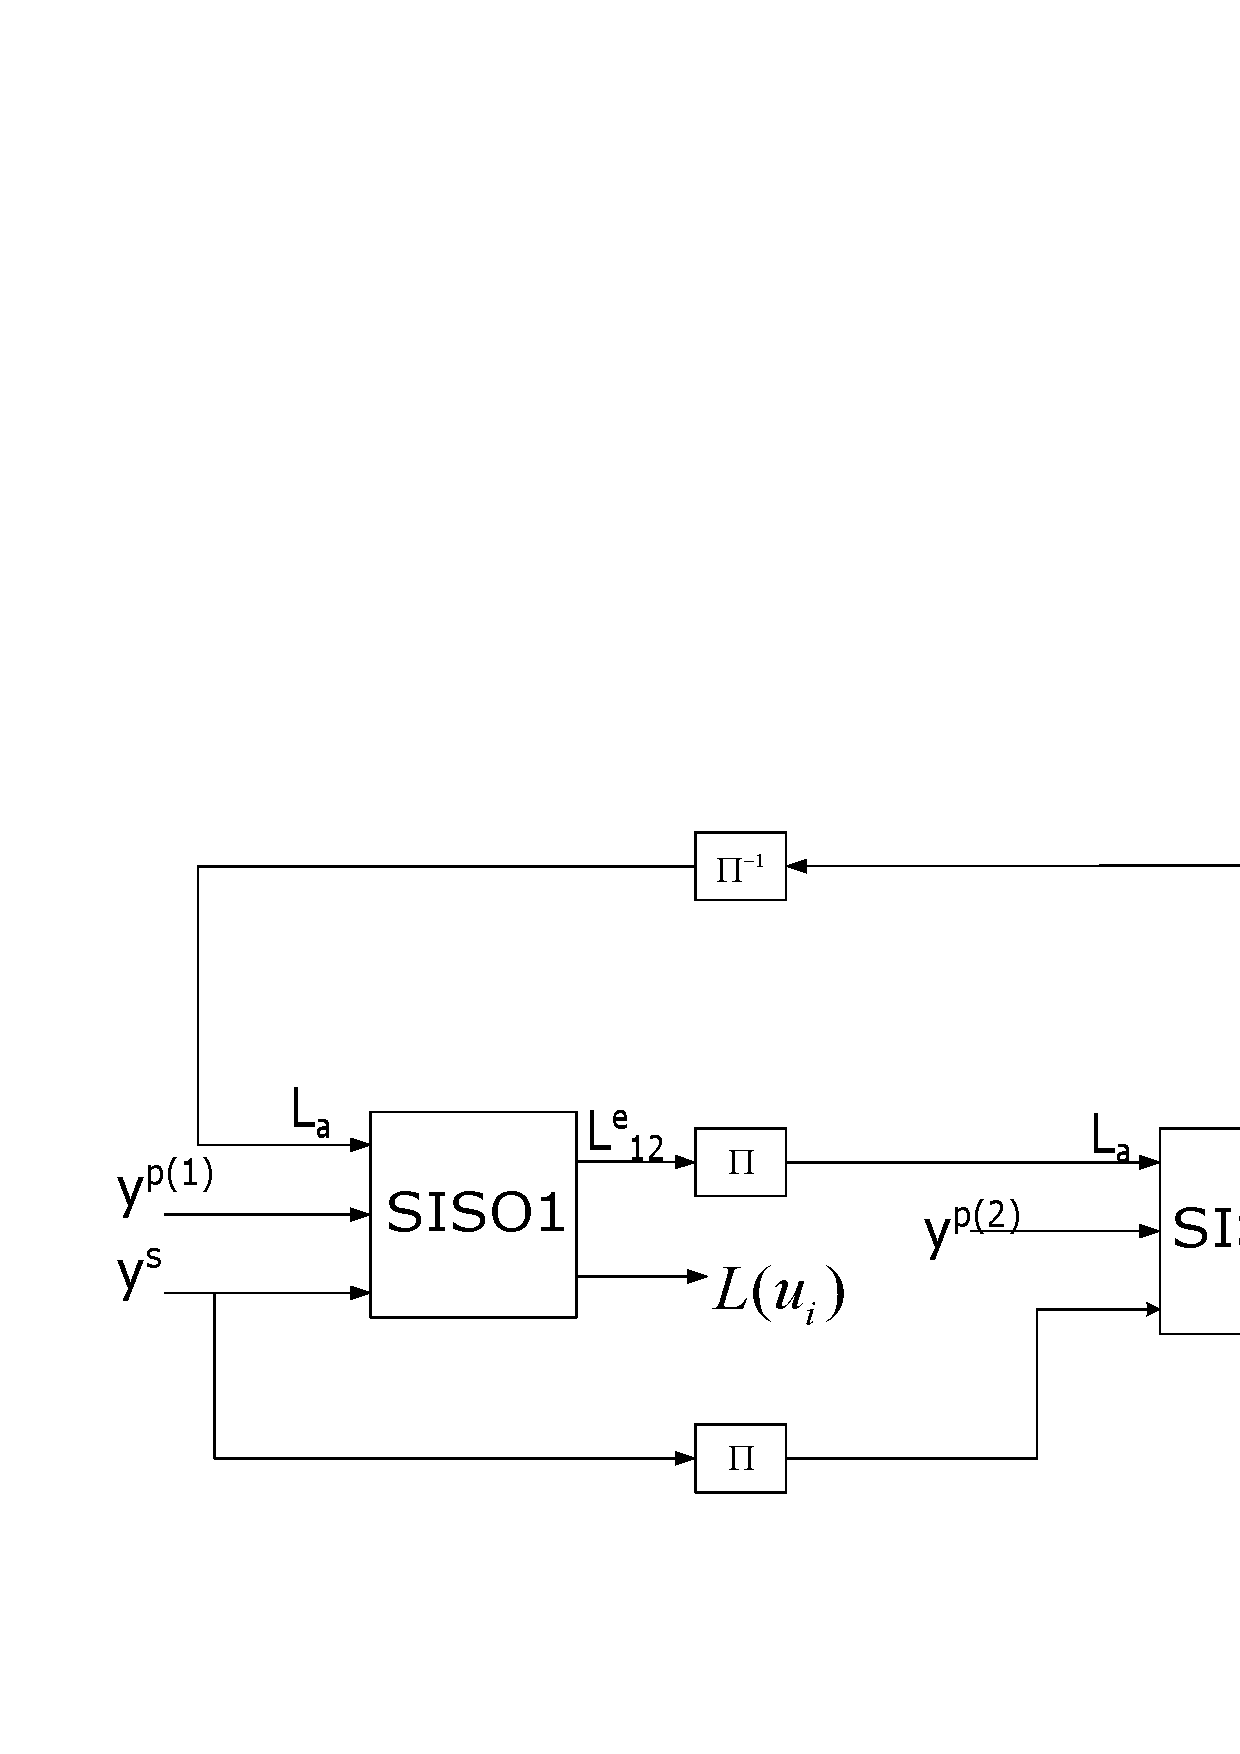
\includegraphics[width=10cm]{D1.pdf}
\caption{Turbo Decoder}
\label{図2}
\end{figure}%
The turbo decoder is shown in figure 1.
To explain the iterative decoding process, the following assumptions are made\paragraph{1}
The component encoders of the Turbo encoder are RSC encoder with rate 1/2\paragraph{2}

 The information bit sequence $\boldsymbol{u}_i=(u_1,u_2,...,u_N)$ is fed into the first RSC encoder and outputs the first parity bit sequence${c}^p=(c_1^p,c_2^p,...,c_N^p)$.\paragraph{3}

 The information bit sequence is fed into the interleaver and outputs、${\boldsymbol{u}'}_i=({u'}_1,{u'}_2,...,{u'}_N)$ which is then fed into the second component encoder to produce the second parity bit sequence、${\boldsymbol{c}'}^p=({c'}_1^p,{c'}_2^p,...,{c'}_N^p)$.

\paragraph{4} $\boldsymbol{u}_i,\boldsymbol{c}^p,{\boldsymbol{c}'}^p$ are BPSK modulated and transmitted over an AWGN channel.\\

\paragraph{5} The received sequence is、$\boldsymbol{y}_i^s,\boldsymbol{y}^p,{\boldsymbol{y}'}_i$ and becomes the input to the decoder.\paragraph{}

The turbo decoding process is as follows
\paragraph{1}
The input to the first component decoder is $(\boldsymbol{y}^s,\boldsymbol{y}^p)$ and relates to the first component encoder of the Turbo encoder.
\paragraph{2}
using equation 17、$L(u_i)$ is calculated. For the first iteration、$u_i$ is assumed to have equal probability and$L^{(a)}(u_i)$ is set to 0。
\paragraph{3}
At the output of the first componet decoder, $L_cy_i^s$ is subtracted from $L(u_i)$ to yield $L_{12}^{(e)}(u_i)$. $L_{12}^{(e)}(u_i)$ is then interleaved and fed into the second component decoder as the value for $L^{(a)}(u_i)$.
\paragraph{4}
The other inputs to the second component decoder are $({\boldsymbol{y}'}^s,{\boldsymbol{y}'}^p)$ and are used to calculate $L_{21}^{(e)}(u_i)$.
\paragraph{5}
$L_{21}^{(e)}(u_i)$ is deinterleaved、and fedback into the first component encoder as the new $L^{(a)}(u_i)$ value.
\paragraph{}
The iteration is either repeated for a predetermined number of times, or untill a certain condition is met. At the final iteration $L(u_i)$ (from the second component decoder)is deinterleaved and used to estimate the value of$u_i$.


\subsection{System Model}
The system model used for the simulation is shown in figure 2. The conditons used for the various sytem blocks are given below。
\begin{figure}[h]
\includegraphics[width=10cm]{figure4.pdf}
\caption{System Model}
\label{}
\end{figure}%
\paragraph{1. \textbf{Turbo Encoder}}
\paragraph{a}
The input to the Turbo encoder is binary.
\paragraph{b}
The component encoders for the Turbo code are  K=3,k=1, n=2 RSC encoders
\paragraph{c}
Quadratic, S-random and Quadratic permutation polynomial interleavers[5] are used. Each one has length ,$2^m$ where the value for  $m$ is within the range ${3 - 10}$, with increments on 1.
\paragraph{d}
output rate of the Turbo encoder is 1/3.
\paragraph{2. BPSK Modulator}\paragraph{}
When the input to the modulator is bit 1 the output is +1, when the input is bit 0, the output is -1.
\paragraph{3. AWGN Channel}\paragraph{}
Zero mean white Gaussian Noise is used. The output SNR is within the range {1 -2} dB with step size of 0.5.
\paragraph{4. Turbo Decoder}\paragraph{}
Quadratic, S-random and Quadratic permutation polynomial interleavers are used. The Max-Log-MAP decoding algorithm is used for the iterative decoding

\section{References}
\paragraph{[1]}   John G. Proakis, Masoud Salehi. ''Digital Communications'', Fifth Edition,Chapter 8, McGraw-Hill\\.
\paragraph{[2]}  Oscar Y. Takeshita, Member, IEEE, and Daniel J. Costello ,''New Deterministic Interleaver Designs for Turbo Codes'',IEEE Trans. Inform. Theory, vol.  46,pp. 1988-2006,Nov. 2000\\
\paragraph{[3]}  L. C. Perez, J. Seghers, D. J. Costello, Jr., ''A distance spectrum interpretation of turbo codes'', IEEE Trans. Inform. Theory, vol. 42, pp. 1698-1709, Nov. 1996.\\
\paragraph{[4]}  C. Berrou, A. Glavieux and P. Thitimajshima, ''Near Shannon limit error-correcting coding and
decoding: Turbo codes'', Proc. Intern. Conf. Communications (ICC), Geneva, Switzerland, pp. 1064-
1070, May 1993. \\
\paragraph{[5]}  Jing Sun, Oscar Y. Takeshita ''Interleavers for Turbo Codes Using Permutation Polynomials over Integer Rings'', IEEE Trans. Inform. Theory, vol. 51, pp. 101 - 119  Jan. 2005\\


\end{document}